\documentclass[12pt,a4paper]{article}
\usepackage[utf8]{vietnam}
\usepackage{amsmath,amssymb,amsfonts,mathrsfs}
\usepackage[left=1.5cm,right=1.5cm,top=2cm,bottom=2cm,headheight=17pt]{geometry}
\usepackage{enumitem}
\usepackage{array}
\usepackage{graphicx}
\usepackage{fancyhdr}

\pagestyle{fancy}
\fancyhf{}
\lhead{\small\textbf{HƯỚNG TỚI THPTQG 2027}}
\rhead{\small\textit{Người biên soạn: Dương Gia Bảo}}
\rfoot{\small Trang \thepage}
\renewcommand{\headrulewidth}{0.4pt}

\begin{document}

\noindent
\begin{minipage}[t]{0.40\textwidth}
    \centering
    \textbf{HƯỚNG TỚI THPTQG 2027}\\[-2pt]
    \rule{3.2cm}{0.6pt}\\[4pt]
    \textbf{ĐỀ CHÍNH THỨC}
\end{minipage}\hfill
\begin{minipage}[t]{0.58\textwidth}
    \centering
    \textbf{ĐỀ THI KHẢO SÁT CHẤT LƯỢNG}\\
    \textbf{ĐỀ SỐ 6}\\
    \textbf{Môn thi: TOÁN}\\
    \textit{\small Thời gian làm bài: 90 phút, không kể thời gian phát đề}
\end{minipage}

\vspace{0.2cm}
\noindent
\begin{minipage}[b]{0.78\textwidth}
    \textbf{Họ và tên:}\dotfill\textbf{SBD:}\makebox[3.5cm]{\dotfill}
\end{minipage}\hfill
\begin{minipage}[b]{0.20\textwidth}
    \hfill
    \setlength{\fboxrule}{0.8pt}%
    \fbox{\begin{minipage}{2.3cm}
        \centering
        \textbf{\small Mã đề thi}\\
        \textbf{0006}
    \end{minipage}}
\end{minipage}
\vspace{0.2cm}

% ==========================================
% PHẦN I
% ==========================================
\section*{\large PHẦN I. CÂU TRẮC NGHIỆM NHIỀU PHƯƠNG ÁN LỰA CHỌN}
\textit{Thí sinh trả lời từ câu 1 đến câu 12. Mỗi câu hỏi thí sinh chỉ chọn một phương án. Mỗi câu trả lời đúng được 0,25 điểm.}

\begin{enumerate}[label=\textbf{Câu \arabic*:}, leftmargin=*]

\item Cho hàm số $y = \dfrac{x^2 - (m+1)x + 2m - 1}{x - m}$. Có bao nhiêu giá trị nguyên của tham số $m \in [-10; 10]$ để đồ thị hàm số có hai điểm cực trị nằm về hai phía đối với trục hoành $Ox$?
\begin{enumerate}[label=\Alph*.]
    \item $4$.
    \item $3$.
    \item $5$.
    \item $18$.
\end{enumerate}

\item Tìm tất cả các giá trị thực của tham số $m$ để bất phương trình $4^x - m \cdot 2^{x+1} + 2m + 3 \le 0$ có nghiệm thực $x \in [0; 2]$.
\begin{enumerate}[label=\Alph*.]
    \item $m \ge 3$.
    \item $m \ge \dfrac{19}{6}$.
    \item $m \le 3$.
    \item $3 \le m \le \dfrac{19}{6}$.
\end{enumerate}

\item Cho hàm số $f(x)$ liên tục trên $\mathbb{R}$ và thỏa mãn $f(x) + f(2-x) = x^3 - 3x^2 + 2x + 4$ với mọi $x \in \mathbb{R}$. Tích phân $I = \int_0^2 f(x) \, \mathrm{d}x$ bằng
\begin{enumerate}[label=\Alph*.]
    \item $I = 8$.
    \item $I = 2$.
    \item $I = 4$.
    \item $I = -4$.
\end{enumerate}

\item Trong không gian $Oxyz$, cho mặt cầu $(S): x^2 + y^2 + z^2 - 2x + 4y - 6z - 2 = 0$ và điểm $A(3; 1; -1)$. Từ $A$ kẻ các tiếp tuyến đến mặt cầu $(S)$, tập hợp các tiếp điểm $M$ tạo thành một đường tròn $(C)$. Bán kính $r$ của đường tròn $(C)$ bằng
\begin{enumerate}[label=\Alph*.]
    \item $r = \sqrt{13}$.
    \item $r = \dfrac{16\sqrt{29}}{29}$.
    \item $r = \dfrac{2\sqrt{29}}{3}$.
    \item $r = \dfrac{4\sqrt{377}}{29}$.
\end{enumerate}

\item Hai người thợ A và B cùng sản xuất độc lập một loại linh kiện điện tử. Xác suất người thợ A tạo ra sản phẩm đạt chuẩn là $0{,}80$, người thợ B tạo ra sản phẩm đạt chuẩn là $0{,}90$. Lấy ngẫu nhiên từ mỗi người 1 sản phẩm để kiểm tra. Biết rằng trong 2 sản phẩm lấy ra có đúng 1 sản phẩm đạt chuẩn, xác suất để sản phẩm đạt chuẩn đó là của người thợ A bằng
\begin{enumerate}[label=\Alph*.]
    \item $\dfrac{9}{13}$.
    \item $\dfrac{4}{13}$.
    \item $0{,}80$.
    \item $\dfrac{1}{4}$.
\end{enumerate}

\item Khảo sát số giờ tự học mỗi tuần của $50$ học sinh lớp 12 thu được bảng số liệu ghép nhóm sau:
\begin{center}
\begin{tabular}{|c|c|c|c|c|}
\hline
\textbf{Số giờ tự học (giờ)} & $[5; 10)$ & $[10; 15)$ & $[15; 20)$ & $[20; 25)$ \\ \hline
\textbf{Số học sinh} & $8$ & $15$ & $17$ & $10$ \\ \hline
\end{tabular}
\end{center}
Khoảng tứ phân vị $\Delta_Q = Q_3 - Q_1$ của mẫu số liệu ghép nhóm trên bằng (làm tròn kết quả đến hàng phần trăm)
\begin{enumerate}[label=\Alph*.]
    \item $7{,}76\text{ giờ}$.
    \item $8{,}75\text{ giờ}$.
    \item $9{,}26\text{ giờ}$.
    \item $6{,}50\text{ giờ}$.
\end{enumerate}

\item Có bao nhiêu giá trị nguyên của tham số $m \in [-10; 10]$ để phương trình $9^x - 2(m+1) \cdot 3^x + 6m - 3 = 0$ có hai nghiệm thực phân biệt $x_1, x_2$ thỏa mãn $x_1 + x_2 > 2$?
\begin{enumerate}[label=\Alph*.]
    \item $9$.
    \item $7$.
    \item $8$.
    \item $10$.
\end{enumerate}

\item Cho hình phẳng $(H)$ giới hạn bởi đồ thị hàm số $y = (x-1)e^x$, trục hoành và hai đường thẳng $x = 0, x = 2$. Thể tích $V$ của khối tròn xoay tạo thành khi quay hình phẳng $(H)$ xung quanh trục $Ox$ bằng
\begin{enumerate}[label=\Alph*.]
    \item $V = \dfrac{e^4 - 5}{4}$.
    \item $V = \dfrac{\pi(e^4 + 1)}{4}$.
    \item $V = \dfrac{\pi(e^4 - 1)}{2}$.
    \item $V = \dfrac{\pi(e^4 - 5)}{4}$.
\end{enumerate}

\item Trong không gian $Oxyz$, cho hai điểm $A(1; 2; -1)$, $B(3; 0; 3)$ và mặt phẳng $(P): x - 2y + 2z - 1 = 0$. Tọa độ điểm $M(a; b; c)$ thuộc mặt phẳng $(P)$ sao cho biểu thức $T = MA^2 + 2MB^2$ đạt giá trị nhỏ nhất. Tổng $a + b + c$ bằng
\begin{enumerate}[label=\Alph*.]
    \item $\dfrac{116}{27}$.
    \item $\dfrac{14}{3}$.
    \item $\dfrac{85}{27}$.
    \item $4$.
\end{enumerate}

\item Cho cấp số nhân $(u_n)$ có tất cả các số hạng đều dương thỏa mãn $u_1 + u_2 + u_3 = 13$ và $\log_3 u_5 - \log_3 u_2 = 3$. Tổng $6$ số hạng đầu tiên $S_6$ của cấp số nhân bằng
\begin{enumerate}[label=\Alph*.]
    \item $728$.
    \item $243$.
    \item $364$.
    \item $121$.
\end{enumerate}

\item Trong không gian $Oxyz$, cho hình hộp $ABCD.A'B'C'D'$ có tọa độ các đỉnh $A(1; 0; 1)$, $B(2; 1; 2)$, $D(1; -1; 0)$ và $C'(4; 5; 6)$. Tọa độ đỉnh $A'$ của hình hộp là
\begin{enumerate}[label=\Alph*.]
    \item $A'(2; 5; 5)$.
    \item $A'(3; 5; 6)$.
    \item $A'(4; 4; 5)$.
    \item $A'(1; 6; 7)$.
\end{enumerate}

\item Một hộp chứa $15$ quả cầu gồm $7$ quả cầu màu đỏ và $8$ quả cầu màu xanh. Lấy ngẫu nhiên đồng thời $4$ quả cầu từ hộp. Tính xác suất để trong $4$ quả cầu lấy ra có ít nhất $1$ quả cầu màu đỏ và số quả cầu màu xanh nhiều hơn số quả cầu màu đỏ.
\begin{enumerate}[label=\Alph*.]
    \item $\dfrac{66}{195}$.
    \item $\dfrac{112}{195}$.
    \item $\dfrac{28}{195}$.
    \item $\dfrac{56}{195}$.
\end{enumerate}

\end{enumerate}

% ==========================================
% PHẦN II
% ==========================================
\section*{PHẦN II. CÂU TRẮC NGHIỆM ĐÚNG/SAI}
\textit{Thí sinh trả lời từ câu 1 đến câu 4. Trong mỗi ý a), b), c), d) ở mỗi câu, thí sinh chọn Đúng hoặc Sai.}

\begin{enumerate}[label=\textbf{Câu \arabic*:}, leftmargin=*]

\item Một xưởng hóa chất sản xuất xút công nghiệp NaOH. Tổng chi phí sản xuất $x$ ngàn tấn sản phẩm trong một tháng ($x > 0$) được mô hình hóa bởi hàm số $C(x) = x^3 - 12x^2 + 60x + 100$ (triệu đồng). Giá bán mỗi ngàn tấn sản phẩm phụ thuộc vào sản lượng cung ứng ra thị trường theo hàm giá $p(x) = 180 - 6x$ (triệu đồng/ngàn tấn). Lợi nhuận ròng thu được là $L(x) = R(x) - C(x)$, trong đó $R(x) = x \cdot p(x)$ là tổng doanh thu.

\begin{enumerate}[label=\alph*)]
    \item Hàm số biểu diễn tổng doanh thu khi xưởng bán $x$ ngàn tấn sản phẩm là $R(x) = 180x - 6x^2$ (triệu đồng).
    \item Khi không bị giới hạn sản lượng, hàm lợi nhuận ròng của xưởng là $L(x) = -x^3 + 6x^2 + 120x - 100$ (triệu đồng) và đạt giá trị lớn nhất tại $x = 2 + 2\sqrt{11} \approx 8{,}63$ ngàn tấn.
    \item Do quy định về hạn ngạch xả thải bảo vệ môi trường, sản lượng tối đa xưởng được phép sản xuất trong tháng là $x \le 6$ ngàn tấn. Mức lợi nhuận lớn nhất xưởng có thể đạt được dưới điều kiện hạn ngạch này vẫn là $739{,}73$ triệu đồng tại $x \approx 8{,}63$ ngàn tấn.
    \item Thực tế dưới điều kiện hạn ngạch môi trường $x \le 6$ ngàn tấn, mức lợi nhuận lớn nhất xưởng đạt được nằm tại điểm biên $x = 6$ ngàn tấn và bằng $620$ triệu đồng.
\end{enumerate}

\item Một cơ sở y tế triển khai quy trình tầm soát bệnh lý di truyền ẩn $X$ trong cộng đồng với tỉ lệ mắc bệnh thực tế là $2\%$ ($P(D) = 0{,}02$). Quy trình kiểm định gồm 2 tầng độc lập:
\begin{itemize}[leftmargin=*]
    \item \textbf{Tầng 1 (Xét nghiệm nhanh)}: Độ nhạy đạt $95\%$ ($P(T_1^+ | D) = 0{,}95$) và độ đặc hiệu đạt $90\%$ ($P(T_1^- | \bar{D}) = 0{,}90$).
    \item \textbf{Tầng 2 (Xét nghiệm PCR chuyên sâu)}: Chỉ thực hiện đối với những người có kết quả $T_1^+$ ở tầng 1. Xét nghiệm PCR có độ nhạy $98\%$ ($P(T_2^+ | D) = 0{,}98$) và độ đặc hiệu $95\%$ ($P(T_2^- | \bar{D}) = 0{,}95$).
\end{itemize}
\begin{center}
    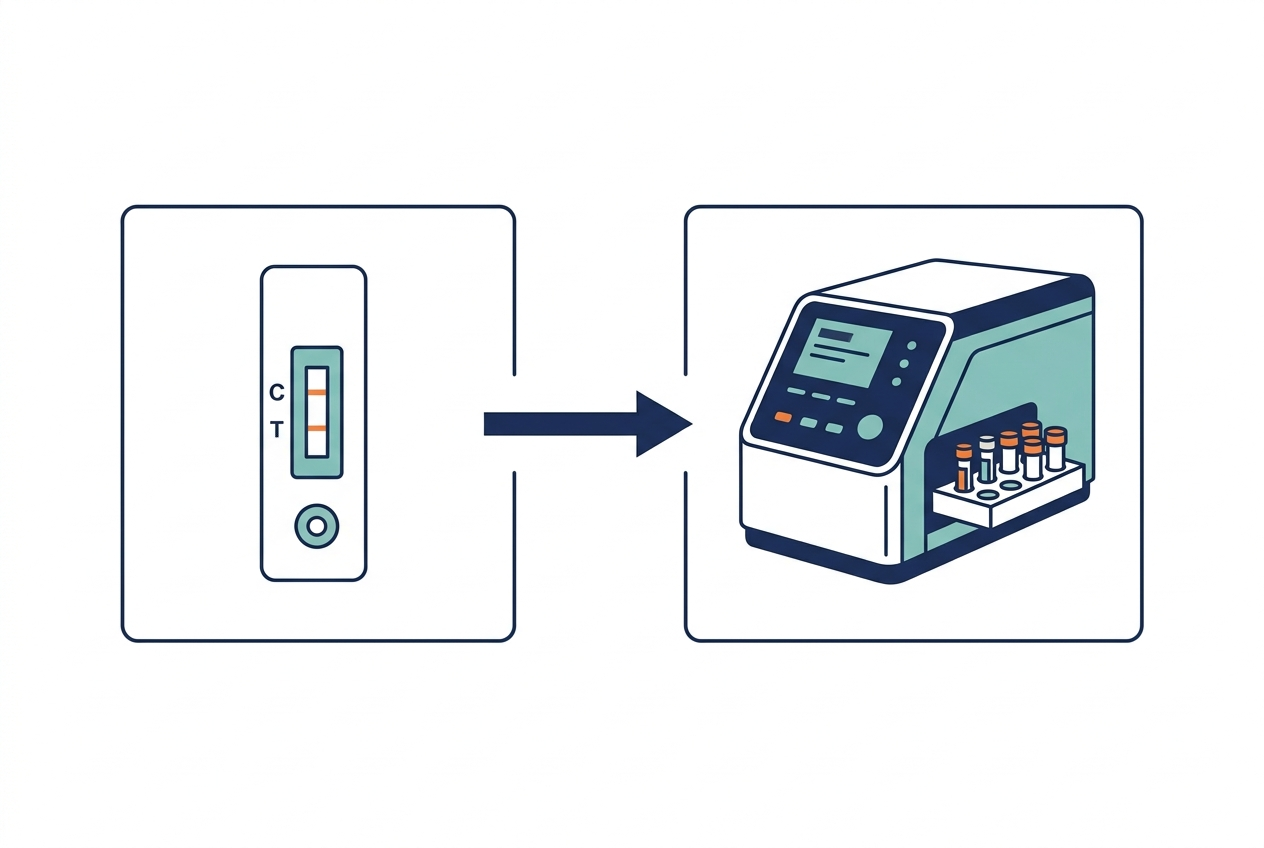
\includegraphics[width=0.42\linewidth,height=3.2cm,keepaspectratio]{images/phan2_cau2_xetnghiem.jpg}
\end{center}
\begin{enumerate}[label=\alph*)]
    \item Xác suất để một người được chọn ngẫu nhiên trong cộng đồng có kết quả dương tính ở Tầng 1 là $P(T_1^+) = 0{,}117$ ($11{,}7\%$).
    \item Biết một người có kết quả dương tính ở Tầng 1, xác suất người đó thực sự mắc bệnh $X$ là $P(D | T_1^+) \approx 16{,}24\%$.
    \item Một kỹ thuật viên nhận định: ``Do xét nghiệm PCR ở Tầng 2 có độ đặc hiệu $95\%$ và độ nhạy $98\%$ rất cao, nên xác suất một người dương tính ở cả 2 tầng thực sự mắc bệnh $X$ sẽ vượt quá $95\%$''.
    \item Xác suất thực tế để một người có kết quả dương tính ở cả 2 tầng xét nghiệm thực sự mắc bệnh $X$ xấp xỉ $79{,}17\%$.
\end{enumerate}

\item Một thiết bị thử nghiệm chuyển động thẳng với gia tốc biến thiên theo thời gian $a(t) = 6t - 18\text{ (m/s}^2\text{)}$ với $t \ge 0$ (giây). Vận tốc ban đầu của vật tại thời điểm $t = 0$ là $v(0) = 24\text{ m/s}$.
\begin{enumerate}[label=\alph*)]
    \item Biểu thức vận tốc của vật thể theo thời gian $t$ là $v(t) = 3t^2 - 18t + 24\text{ (m/s)}$.
    \item Trong khoảng thời gian từ $t = 0$ đến $t = 2$ giây, vật thể chuyển động theo chiều dương và đi được quãng đường $s_1 = 20\text{ m}$.
    \item Độ dời của vật tại thời điểm $t = 4$ giây so với vị trí ban đầu $t = 0$ là $16\text{ m}$. Từ đó kết luận quãng đường vật đi được trong 4 giây đầu tiên bằng $16\text{ m}$.
    \item Tổng quãng đường thực tế mà vật thể đi được trong 4 giây đầu tiên kể từ $t = 0$ bằng $24\text{ m}$.
\end{enumerate}

\item \begin{minipage}[t]{0.55\linewidth}
Trong không gian $Oxyz$ (đơn vị đo là mét), hai thiết bị bay không người lái (drone) $A$ và $B$ cất cánh đồng thời tại thời điểm $t = 0$ (giây):
\begin{itemize}[leftmargin=*]
    \item Drone $A$ xuất phát từ $A_0(1; 2; 5)$ bay thẳng đều với vectơ vận tốc $\vec{v}_A = (2; 1; -1)\text{ (m/s)}$.
    \item Drone $B$ xuất phát từ $B_0(10; -5; 2)$ bay thẳng đều với vectơ vận tốc $\vec{v}_B = (-1; 4; 2)\text{ (m/s)}$.
\end{itemize}
\begin{enumerate}[label=\alph*)]
    \item Tại thời điểm $t = 1$ giây, tọa độ vị trí của hai drone lần lượt là $A(3; 3; 4)$ và $B(9; -1; 4)$.
    \item Khoảng cách giữa hai drone tại thời điểm $t \ge 0$ được xác định bởi hàm số $d(t) = \sqrt{27t^2 - 114t + 139}\text{ (m)}$.
    \item Trong một đợt kiểm thử bị giới hạn thời gian bay $t \in [0; 1{,}5]$ giây, kỹ thuật viên kết luận khoảng cách ngắn nhất giữa hai drone đạt được tại $t = \dfrac{19}{9} \approx 2{,}11$ giây với giá trị $d \approx 4{,}32\text{ m}$.
    \item Thực tế trong khoảng thời gian kiểm thử $t \in [0; 1{,}5]$ giây, khoảng cách ngắn nhất giữa hai drone đạt được tại thời điểm biên $t = 1{,}5$ giây và bằng $d = \sqrt{28{,}75} \approx 5{,}36\text{ m}$.
\end{enumerate}
\end{minipage}\hfill
\begin{minipage}[t]{0.42\linewidth}
\vspace{-0.7\baselineskip}
\centering
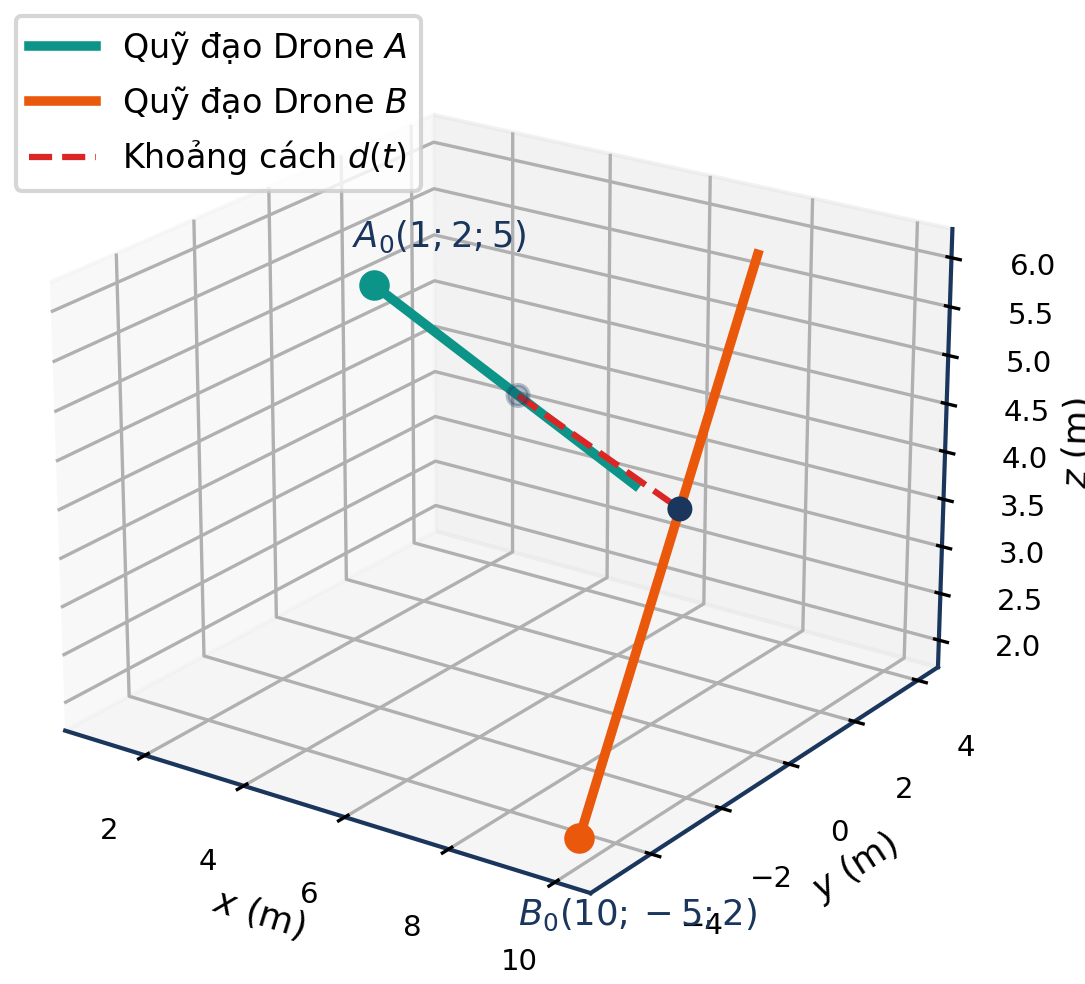
\includegraphics[width=\linewidth]{images/phan2_cau4_haidrone_3d.png}
\end{minipage}

\end{enumerate}

% ==========================================
% PHẦN III
% ==========================================
\section*{PHẦN III. CÂU TRẮC NGHIỆM TRẢ LỜI NGẮN}
\textit{Thí sinh trả lời từ câu 1 đến câu 6. Điền đáp số theo quy chuẩn làm tròn được nêu trong từng câu.}

\begin{enumerate}[label=\textbf{Câu \arabic*:}, leftmargin=*]

\item \begin{minipage}[t]{0.57\linewidth}
Một công ty năng lượng thiết kế một bể chứa nhiên liệu công nghiệp hình hộp chữ nhật không nắp có thể tích cố định $V = 128\text{ m}^3$. Đáy bể là hình chữ nhật có chiều dài gấp $2$ lần chiều rộng (gọi chiều rộng đáy là $x\text{ (m)}$, $x > 0$). Chi phí vật liệu chế tạo đáy bể là $300.000\text{ đồng/m}^2$, chi phí vật liệu làm hai mặt bên chiều rộng là $200.000\text{ đồng/m}^2$, và chi phí làm hai mặt bên chiều dài là $200.000\text{ đồng/m}^2$. Tìm chiều rộng $x$ (mét) của đáy bể để tổng chi phí vật liệu chế tạo bể chứa là nhỏ nhất.
\end{minipage}\hfill
\begin{minipage}[t]{0.40\linewidth}
\vspace{-0.7\baselineskip}
\centering
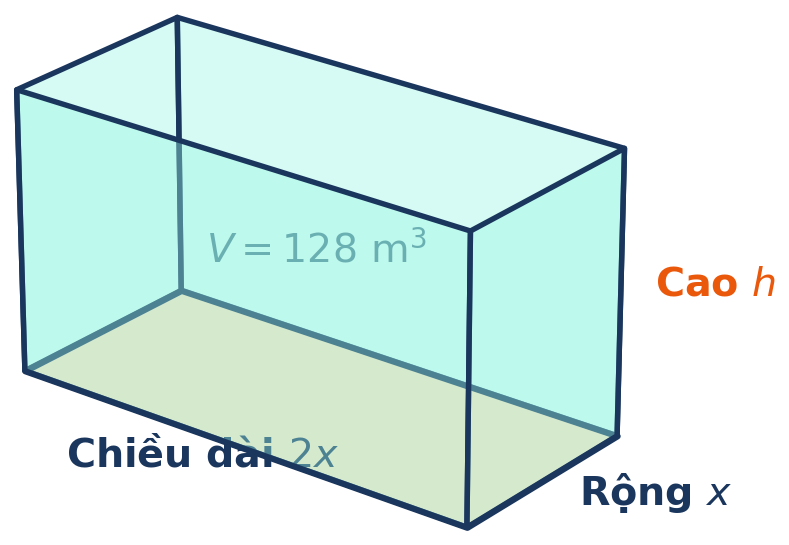
\includegraphics[width=0.95\linewidth]{images/phan3_cau1_bechua_3d.png}
\end{minipage}

\item \begin{minipage}[t]{0.57\linewidth}
Cho hình chóp $S.ABCD$ có đáy $ABCD$ là hình vuông cạnh $a = 6$, cạnh bên $SA$ vuông góc với mặt phẳng đáy $(ABCD)$. Gọi $h$ là chiều cao $SA$ của hình chóp. Biết rằng khoảng cách giữa hai đường thẳng chéo nhau $SC$ và $BD$ bằng $2\sqrt{3}$. Tính chiều cao $h = SA$ của hình chóp.
\end{minipage}\hfill
\begin{minipage}[t]{0.40\linewidth}
\vspace{-0.7\baselineskip}
\centering
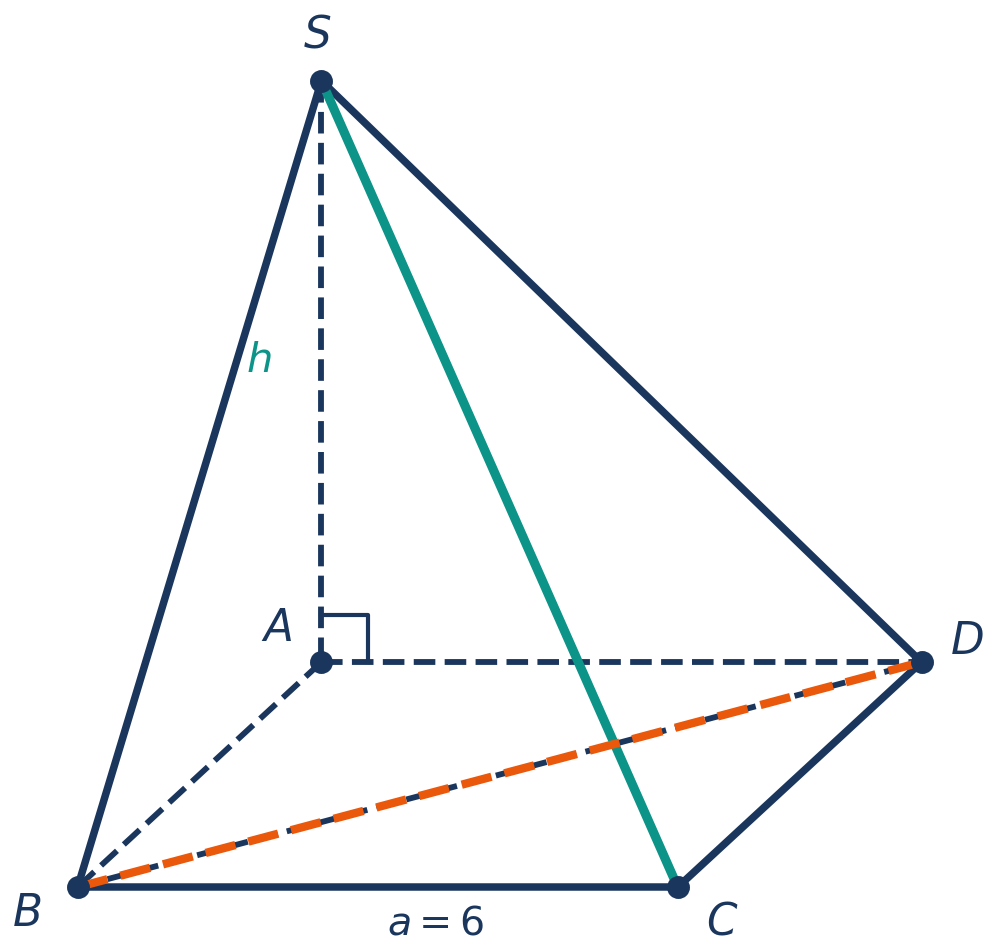
\includegraphics[width=0.88\linewidth]{images/phan3_cau2_hinhchop.png}
\end{minipage}

\item \begin{minipage}[t]{0.55\linewidth}
Hai robot tự hành $A$ và $B$ xuất phát đồng thời tại thời điểm $t = 0$ (giây) và chuyển động trên hai trục tọa độ vuông góc $Ox$ và $Oy$ (đơn vị đo là mét):
\begin{itemize}[leftmargin=*]
    \item Robot $A$ di chuyển trên trục $Ox$ với vị trí được xác định bởi $x(t) = 6 - 2t\text{ (m)}$.
    \item Robot $B$ di chuyển trên trục $Oy$ với vận tốc $v_B(t) = 2e^t\text{ (m/s)}$ và vị trí ban đầu $y(0) = 0\text{ (m)}$ (suy ra vị trí tại thời điểm $t$ là $y(t) = 2e^t - 2$).
\end{itemize}
Tính khoảng cách ngắn nhất giữa hai robot trong quá trình chuyển động với $t \ge 0$ (làm tròn kết quả đến hàng phần trăm).
\end{minipage}\hfill
\begin{minipage}[t]{0.42\linewidth}
\vspace{-0.7\baselineskip}
\centering
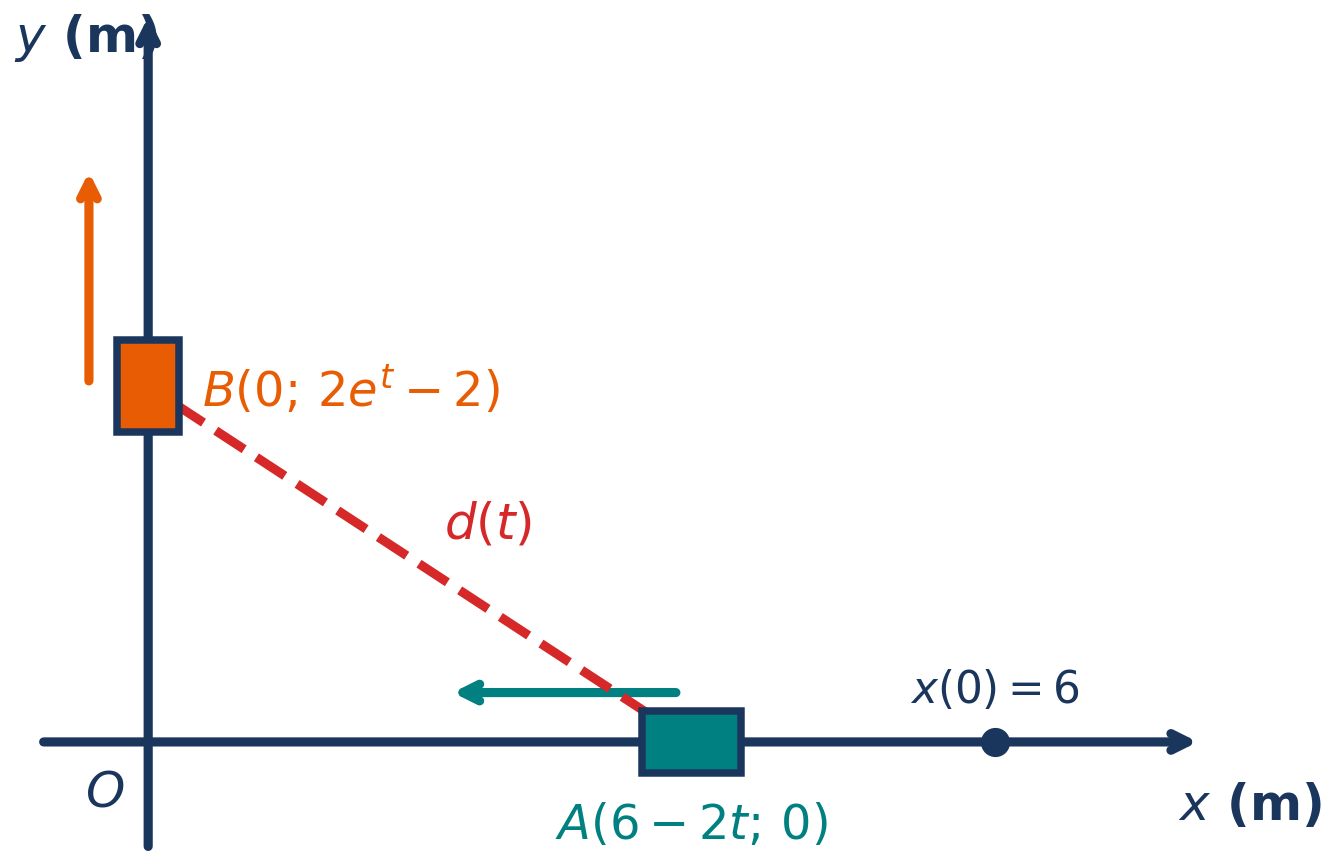
\includegraphics[width=\linewidth]{images/phan3_cau3_hairobot_oxy.png}
\end{minipage}

\item \begin{minipage}[t]{0.57\linewidth}
Trong không gian $Oxyz$, một nguồn sáng điểm $S(0; 0; 12)$ chiếu ánh sáng xuống mặt phẳng đất $Oxy$ ($z = 0$). Một đĩa tròn mỏng có bán kính $R = 2\text{ m}$ nằm song song với mặt phẳng $Oxy$, có tâm $C(0; 0; z(t))$ di chuyển thẳng đứng xuống dưới theo chiều âm của trục $Oz$ với tốc độ không đổi $v = 1{,}5\text{ m/s}$. Bóng của đĩa tròn trên mặt đất $Oxy$ là một hình tròn có diện tích $S(t)$. Tại thời điểm đĩa tròn ở độ cao $z = 6\text{ m}$, tốc độ thay đổi diện tích bóng của đĩa tròn trên mặt đất bằng $k\pi\text{ (m}^2/\text{s)}$. Tìm giá trị của $k$.
\end{minipage}\hfill
\begin{minipage}[t]{0.40\linewidth}
\vspace{-0.7\baselineskip}
\centering
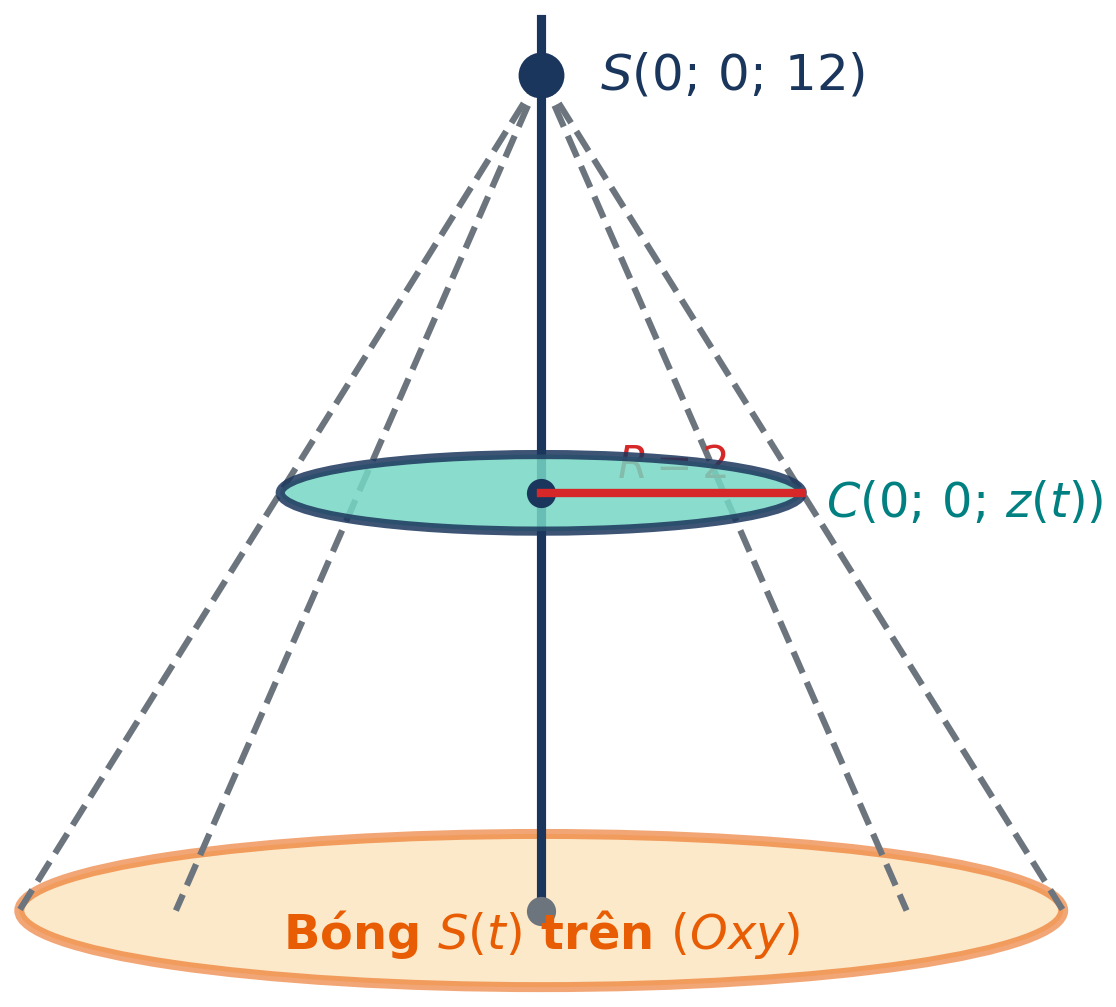
\includegraphics[width=0.92\linewidth]{images/phan3_cau4_nonanhsang.png}
\end{minipage}

\item Hai xạ thủ $A$ và $B$ tham gia một trò chơi bắn súng đối kháng lặp lại vô hạn lượt cho đến khi có người bắn trúng mục tiêu đầu tiên thì trò chơi dừng lại. Xạ thủ $A$ thực hiện phát bắn trước với xác suất bắn trúng mục tiêu trong mỗi lần bắn là $p_1 = \dfrac{1}{4}$. Xạ thủ $B$ thực hiện phát bắn sau với xác suất bắn trúng mục tiêu trong mỗi lần bắn là $p_2 = \dfrac{2}{5}$. Tính xác suất để xạ thủ $A$ là người chiến thắng (bắn trúng mục tiêu trước). Kết quả được biểu diễn dưới dạng phân số tối giản $\dfrac{a}{b}$ với $a, b \in \mathbb{N}^*$. Tính giá trị biểu thức $T = a + b$.
\begin{center}
    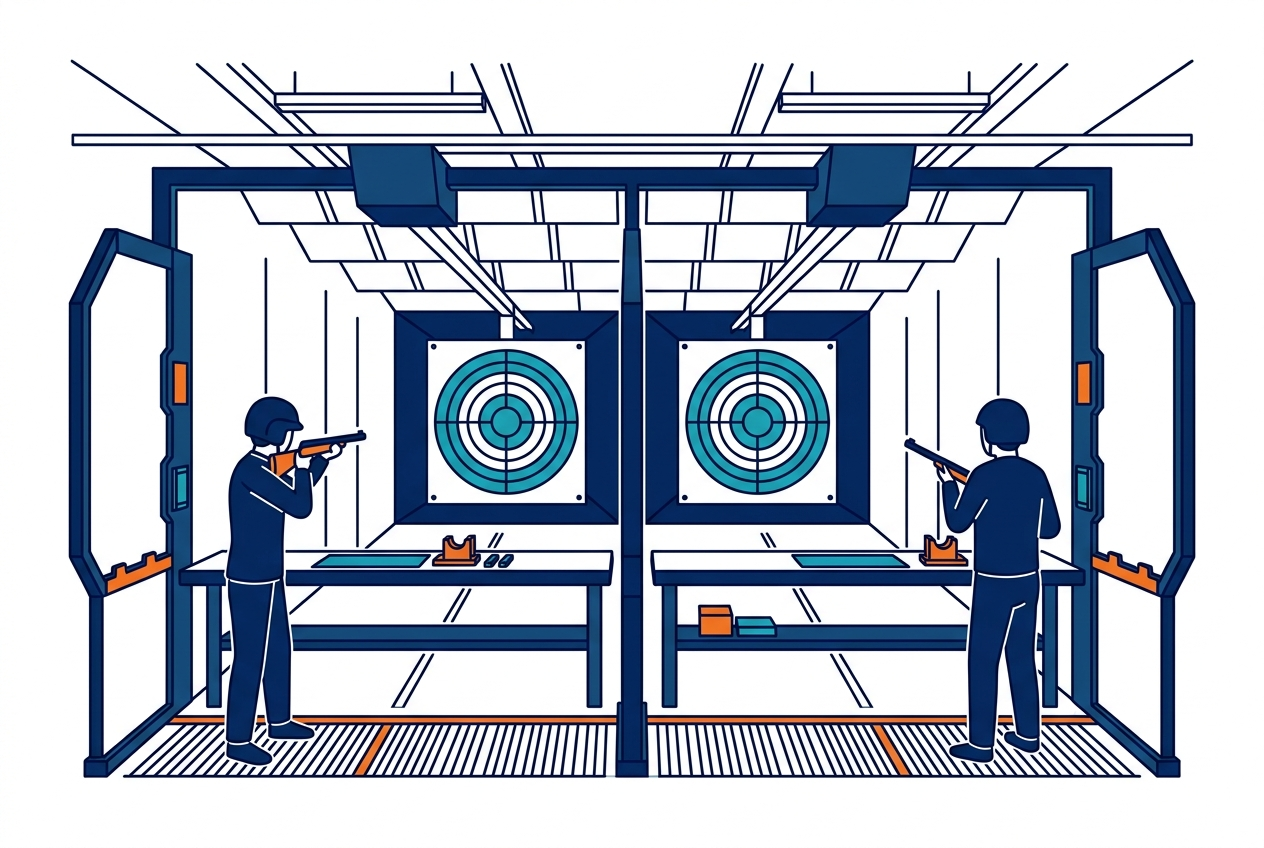
\includegraphics[width=0.42\linewidth,height=3.2cm,keepaspectratio]{images/phan3_cau5_bansung.jpg}
\end{center}

\item \begin{minipage}[t]{0.55\linewidth}
Một mô hình trang trí kiến trúc nghệ thuật $K$ nằm giữa hai mặt phẳng vuông góc với trục $Ox$ tại $x = 0$ và $x = 2$ (đơn vị đo là mét). Cắt mô hình $K$ bởi mặt phẳng vuông góc với trục $Ox$ tại điểm có hoành độ $x$ ($0 \le x \le 2$), thiết diện thu được là một hình tam giác vuông có hai cạnh góc vuông:
\begin{itemize}[leftmargin=*]
    \item Cạnh thứ nhất nằm trên mặt phẳng $Oxy$, có độ dài $b(x) = x e^x - x^2\text{ (m)}$.
    \item Cạnh thứ hai vuông góc với mặt phẳng $Oxy$, có độ dài $h(x) = 2 e^{-x}\text{ (m)}$.
\end{itemize}
Thể tích $V$ của mô hình $K$ được viết dưới dạng $V = a \cdot e^{-b}\text{ (m}^3)$ với $a, b \in \mathbb{N}^*$. Tính giá trị của biểu thức $T = a + b$.
\end{minipage}\hfill
\begin{minipage}[t]{0.42\linewidth}
\vspace{-0.7\baselineskip}
\centering
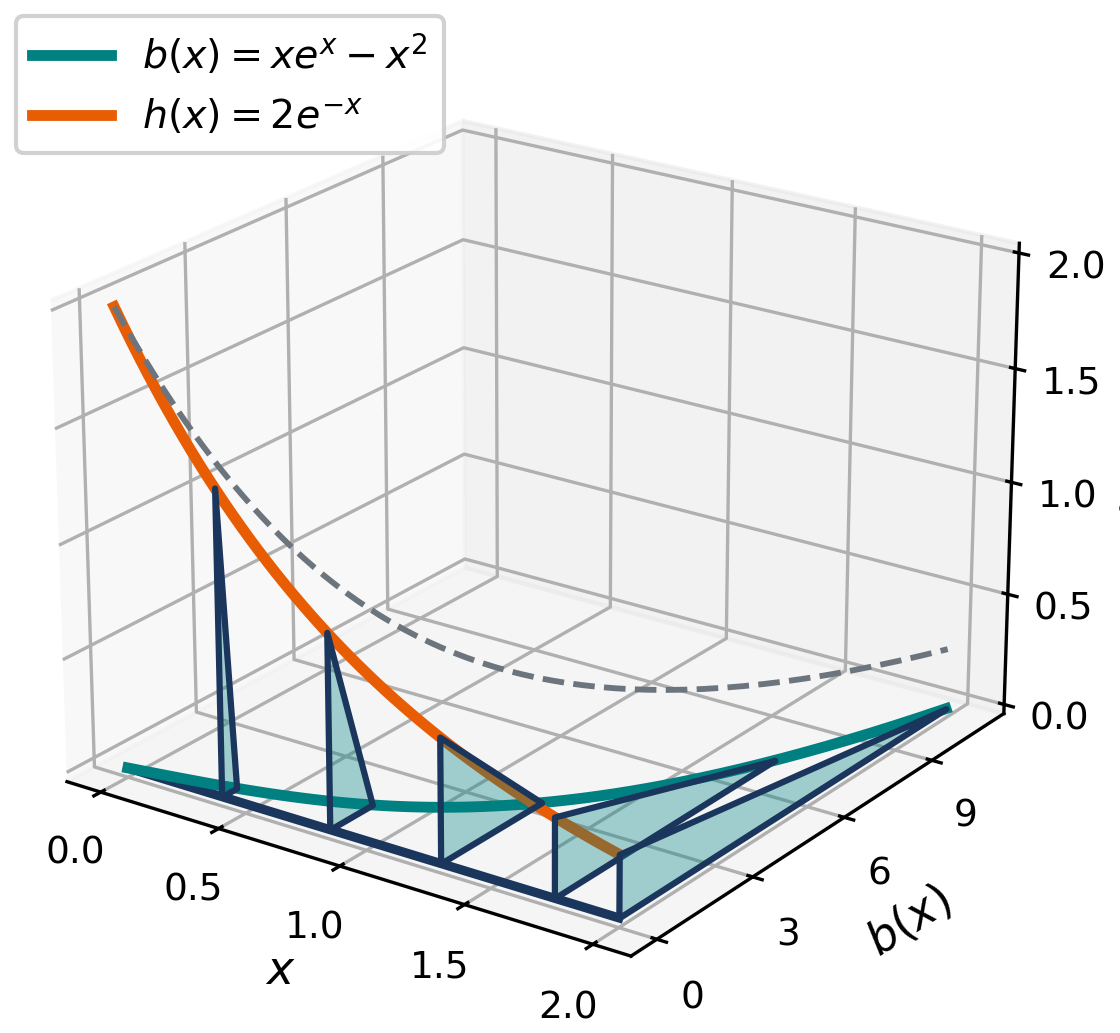
\includegraphics[width=\linewidth]{images/phan3_cau6_thietdien_3d.png}
\end{minipage}

\end{enumerate}

\newpage
% ==========================================
% BẢNG ĐÁP ÁN TỔNG HỢP
% ==========================================
\section*{BẢNG ĐÁP ÁN TỔNG HỢP}

\subsection*{1. PHẦN I}
\begin{center}
\begin{tabular}{|c|c||c|c||c|c||c|c|}
\hline
\textbf{Câu} & \textbf{Đáp án} & \textbf{Câu} & \textbf{Đáp án} & \textbf{Câu} & \textbf{Đáp án} & \textbf{Câu} & \textbf{Đáp án} \\ \hline
1 & B & 4 & D & 7 & C & 10 & C \\ \hline
2 & A & 5 & B & 8 & D & 11 & B \\ \hline
3 & C & 6 & A & 9 & A & 12 & D \\ \hline
\end{tabular}
\end{center}

\subsection*{2. PHẦN II}
\begin{center}
\begin{tabular}{|c|c|c|c|c|}
\hline
\textbf{Câu} & \textbf{Ý a)} & \textbf{Ý b)} & \textbf{Ý c)} & \textbf{Ý d)} \\ \hline
\textbf{1} & Đúng & Đúng & Sai & Đúng \\ \hline
\textbf{2} & Đúng & Đúng & Sai & Đúng \\ \hline
\textbf{3} & Đúng & Đúng & Sai & Đúng \\ \hline
\textbf{4} & Đúng & Đúng & Sai & Đúng \\ \hline
\end{tabular}
\end{center}

\subsection*{3. PHẦN III}
\begin{center}
\begin{tabular}{|c|c||c|c||c|c|}
\hline
\textbf{Câu} & \textbf{Kết quả điền} & \textbf{Câu} & \textbf{Kết quả điền} & \textbf{Câu} & \textbf{Kết quả điền} \\ \hline
\textbf{1} & 4 & \textbf{3} & 5,02 & \textbf{5} & 16 \\ \hline
\textbf{2} & 12 & \textbf{4} & 8 & \textbf{6} & 12 \\ \hline
\end{tabular}
\end{center}

\newpage
% ==========================================
% HƯỚNG DẪN GIẢI CHI TIẾT
% ==========================================
\section*{HƯỚNG DẪN GIẢI CHI TIẾT}

\subsection*{PHẦN I}
\begin{enumerate}[label=\textbf{Câu \arabic*:}, leftmargin=*]
\item \textbf{Đáp án B.}
Tập xác định: $D = \mathbb{R} \setminus \{m\}$.\\
Chia đa thức: $x^2 - (m+1)x + 2m - 1 = (x - m)(x - 1) + m - 1 \implies y = x - 1 + \dfrac{m - 1}{x - m}$.\\
Đạo hàm: $y' = 1 - \dfrac{m - 1}{(x - m)^2} = \dfrac{(x - m)^2 - (m - 1)}{(x - m)^2}$.\\
Để hàm số có hai điểm cực trị thì $m - 1 > 0 \iff m > 1$.\\
Khi đó hoành độ 2 điểm cực trị là $x = m \pm \sqrt{m - 1}$.\\
Phương trình đường thẳng đi qua hai điểm cực trị là đạo hàm tử trên đạo hàm mẫu:
$$y = \dfrac{2x - (m + 1)}{1} = 2x - m - 1.$$
Tọa độ hai điểm cực trị là:
\begin{align*}
y_1 &= 2(m - \sqrt{m - 1}) - m - 1 = m - 1 - 2\sqrt{m - 1}, \\
y_2 &= 2(m + \sqrt{m - 1}) - m - 1 = m - 1 + 2\sqrt{m - 1}.
\end{align*}
Hai điểm cực trị nằm về hai phía trục hoành khi và chỉ khi:
$$y_1 y_2 < 0 \iff (m - 1)^2 - 4(m - 1) < 0 \iff (m - 1)(m - 5) < 0 \iff 1 < m < 5.$$
Vì $m \in \mathbb{Z}$ và $m \in [-10; 10]$ nên $m \in \{2; 3; 4\}$. Có đúng $3$ giá trị nguyên thỏa mãn.

\item \textbf{Đáp án A.}
Đặt $t = 2^x$. Vì $x \in [0; 2]$ nên $t \in [1; 4]$.\\
Bất phương trình trở thành:
$$t^2 - 2mt + 2m + 3 \le 0 \iff t^2 + 3 \le 2m(t - 1).$$
Với $t = 1$, ta có $1^2 + 3 = 4 \le 0$ (vô lý).\\
Với $t \in (1; 4]$, chia hai vế cho $t - 1 > 0$:
$$2m \ge \dfrac{t^2 + 3}{t - 1} = g(t).$$
Bất phương trình có nghiệm trên $[0; 2] \iff 2m \ge \min\limits_{(1; 4]} g(t)$.\\
Đạo hàm: $g'(t) = \dfrac{2t(t - 1) - (t^2 + 3)}{(t - 1)^2} = \dfrac{t^2 - 2t - 3}{(t - 1)^2} = \dfrac{(t - 3)(t + 1)}{(t - 1)^2}$.\\
Trên $(1; 4]$, $g'(t) = 0 \iff t = 3$. Lập bảng biến thiên thấy $g(t)$ đạt cực tiểu tại $t = 3$ với giá trị:
$$g(3) = \dfrac{3^2 + 3}{3 - 1} = \dfrac{12}{2} = 6.$$
Do đó điều kiện để bất phương trình có nghiệm là: $2m \ge 6 \iff m \ge 3$.

\item \textbf{Đáp án C.}
Đặt $t = 2 - x \implies \mathrm{d}x = -\mathrm{d}t$. Khi $x = 0 \implies t = 2$; khi $x = 2 \implies t = 0$.\\
Suy ra:
$$I = \int_0^2 f(x) \mathrm{d}x = \int_0^2 f(2 - t) \mathrm{d}t = \int_0^2 f(2 - x) \mathrm{d}x.$$
Cộng hai vế lại ta được:
$$2I = \int_0^2 \left[ f(x) + f(2 - x) \right] \mathrm{d}x = \int_0^2 (x^3 - 3x^2 + 2x + 4) \mathrm{d}x.$$
Tính tích phân:
$$2I = \left[ \dfrac{x^4}{4} - x^3 + x^2 + 4x \right]_0^2 = \left( 4 - 8 + 4 + 8 \right) = 8 \implies I = 4.$$

\item \textbf{Đáp án D.}
Mặt cầu $(S)$ có tâm $I(1; -2; 3)$ và bán kính $R = \sqrt{1^2 + (-2)^2 + 3^2 - (-2)} = \sqrt{16} = 4$.\\
Khoảng cách từ điểm $A(3; 1; -1)$ đến tâm $I$ là:
$$IA = \sqrt{(3 - 1)^2 + (1 - (-2))^2 + (-1 - 3)^2} = \sqrt{4 + 9 + 16} = \sqrt{29}.$$
Vì $IA = \sqrt{29} > R = 4$, điểm $A$ nằm ngoài mặt cầu.\\
Độ dài tiếp tuyến kẻ từ $A$ đến mặt cầu là:
$$AM = \sqrt{IA^2 - R^2} = \sqrt{29 - 16} = \sqrt{13}.$$
Bán kính đường tròn tiếp điểm $(C)$ là đường cao trong tam giác vuông $IMA$ vuông tại $M$:
$$r = \dfrac{IM \cdot AM}{IA} = \dfrac{4 \cdot \sqrt{13}}{\sqrt{29}} = \dfrac{4\sqrt{377}}{29}.$$

\item \textbf{Đáp án B.}
Gọi $A_{\text{đ}}$ là biến cố thợ A làm ra sản phẩm đạt chuẩn ($P(A_{\text{đ}}) = 0{,}80$), $B_{\text{đ}}$ là biến cố thợ B làm ra sản phẩm đạt chuẩn ($P(B_{\text{đ}}) = 0{,}90$).\\
Gọi $E$ là biến cố ``Trong 2 sản phẩm lấy ra có đúng 1 sản phẩm đạt chuẩn'':
$$P(E) = P(A_{\text{đ}})P(\overline{B_{\text{đ}}}) + P(\overline{A_{\text{đ}}})P(B_{\text{đ}}) = 0{,}80 \times (1 - 0{,}90) + (1 - 0{,}80) \times 0{,}90 = 0{,}08 + 0{,}18 = 0{,}26.$$
Xác suất để sản phẩm đạt chuẩn đó là của thợ A là xác suất có điều kiện:
$$P(A_{\text{đ}} | E) = \dfrac{P(A_{\text{đ}} \cap \overline{B_{\text{đ}}})}{P(E)} = \dfrac{0{,}08}{0{,}26} = \dfrac{4}{13}.$$

\item \textbf{Đáp án A.}
Cỡ mẫu $N = 8 + 15 + 17 + 10 = 50$.\\
- Tứ phân vị thứ nhất $Q_1$: $\dfrac{N}{4} = 12{,}5$. Tần số tích lũy nhóm 1 là 8; nhóm 2 là $23 \ge 12{,}5$. Do đó nhóm chứa $Q_1$ là $[10; 15)$:
$$Q_1 = 10 + \dfrac{12{,}5 - 8}{15} \times (15 - 10) = 10 + \dfrac{4{,}5}{3} = 11{,}5\text{ giờ}.$$
- Tứ phân vị thứ ba $Q_3$: $\dfrac{3N}{4} = 37{,}5$. Nhóm 3 có tích lũy trước là 23, tích lũy đến nhóm 3 là $40 \ge 37{,}5$. Do đó nhóm chứa $Q_3$ là $[15; 20)$:
$$Q_3 = 15 + \dfrac{37{,}5 - 23}{17} \times (20 - 15) = 15 + \dfrac{14{,}5 \times 5}{17} = 15 + \dfrac{72{,}5}{17} \approx 19{,}2647\text{ giờ}.$$
Khoảng tứ phân vị:
$$\Delta_Q = Q_3 - Q_1 \approx 19{,}2647 - 11{,}5 \approx 7{,}76\text{ giờ}.$$

\item \textbf{Đáp án C.}
Đặt $t = 3^x > 0$. Phương trình trở thành:
$$t^2 - 2(m + 1)t + 6m - 3 = 0.$$
Ta có $\Delta' = (m + 1)^2 - (6m - 3) = m^2 - 4m + 4 = (m - 2)^2 \ge 0$.\\
Để phương trình có hai nghiệm thực phân biệt thì $\Delta' > 0 \iff m \ne 2$.\\
Khi đó hai nghiệm là:
$$t_1 = (m + 1) - (m - 2) = 3,\quad t_2 = (m + 1) + (m - 2) = 2m - 1.$$
Vì $t_1 = 3 > 0 \implies x_1 = 1$.\\
Để phương trình có 2 nghiệm phân biệt thì $t_2 > 0$ và $t_2 \ne t_1 \iff 2m - 1 > 0$ và $2m - 1 \ne 3 \iff m > \dfrac{1}{2}$ và $m \ne 2$.\\
Yêu cầu $x_1 + x_2 > 2 \iff 1 + x_2 > 2 \iff x_2 > 1 \iff t_2 > 3 \iff 2m - 1 > 3 \iff m > 2$.\\
Kết hợp với $m \in \mathbb{Z}$ và $m \in [-10; 10]$, ta được $m \in \{3; 4; 5; 6; 7; 8; 9; 10\}$. Có đúng $8$ giá trị nguyên.

\item \textbf{Đáp án D.}
Thể tích khối tròn xoay là:
$$V = \pi \int_0^2 (x - 1)^2 e^{2x} \mathrm{d}x.$$
Đặt $\begin{cases} u = (x - 1)^2 \\ \mathrm{d}v = e^{2x} \mathrm{d}x \end{cases} \implies \begin{cases} \mathrm{d}u = 2(x - 1) \mathrm{d}x \\ v = \dfrac{1}{2} e^{2x} \end{cases}$.\\
Áp dụng công thức tích phân từng phần:
$$\int_0^2 (x - 1)^2 e^{2x} \mathrm{d}x = \left[ \dfrac{(x - 1)^2 e^{2x}}{2} \right]_0^2 - \int_0^2 (x - 1) e^{2x} \mathrm{d}x = \left( \dfrac{e^4}{2} - \dfrac{1}{2} \right) - \int_0^2 (x - 1) e^{2x} \mathrm{d}x.$$
Tiếp tục tích phân từng phần:
$$\int_0^2 (x - 1) e^{2x} \mathrm{d}x = \left[ \dfrac{(x - 1) e^{2x}}{2} \right]_0^2 - \int_0^2 \dfrac{e^{2x}}{2} \mathrm{d}x = \left( \dfrac{e^4}{2} + \dfrac{1}{2} \right) - \left[ \dfrac{e^{2x}}{4} \right]_0^2 = \dfrac{e^4 + 3}{4}.$$
Suy ra:
$$\int_0^2 (x - 1)^2 e^{2x} \mathrm{d}x = \dfrac{e^4 - 1}{2} - \dfrac{e^4 + 3}{4} = \dfrac{e^4 - 5}{4} \implies V = \dfrac{\pi(e^4 - 5)}{4}.$$

\item \textbf{Đáp án A.}
Tìm điểm $I$ thỏa mãn $\overrightarrow{IA} + 2\overrightarrow{IB} = \vec{0} \implies I = \dfrac{A + 2B}{3}$.\\
Tọa độ điểm $I$:
$$x_I = \dfrac{1 + 2(3)}{3} = \dfrac{7}{3},\quad y_I = \dfrac{2 + 2(0)}{3} = \dfrac{2}{3},\quad z_I = \dfrac{-1 + 2(3)}{3} = \dfrac{5}{3} \implies I\left(\dfrac{7}{3}; \dfrac{2}{3}; \dfrac{5}{3}\right).$$
Khi đó $T = MA^2 + 2MB^2 = 3MI^2 + IA^2 + 2IB^2$.\\
Biểu thức $T$ đạt giá trị nhỏ nhất khi và chỉ khi khoảng cách $MI$ nhỏ nhất, tức $M$ là hình chiếu vuông góc của $I$ lên $(P)$.\\
Đường thẳng đi qua $I$ vuông góc với $(P)$ có phương trình tham số:
$$x = \dfrac{7}{3} + t,\quad y = \dfrac{2}{3} - 2t,\quad z = \dfrac{5}{3} + 2t.$$
Thay vào $(P): x - 2y + 2z - 1 = 0$:
$$\left(\dfrac{7}{3} + t\right) - 2\left(\dfrac{2}{3} - 2t\right) + 2\left(\dfrac{5}{3} + 2t\right) - 1 = 0 \iff 9t + \dfrac{10}{3} = 0 \iff t = -\dfrac{10}{27}.$$
Tọa độ điểm $M(a; b; c)$:
$$a = \dfrac{7}{3} - \dfrac{10}{27} = \dfrac{53}{27},\quad b = \dfrac{2}{3} + \dfrac{20}{27} = \dfrac{38}{27},\quad c = \dfrac{5}{3} - \dfrac{20}{27} = \dfrac{25}{27}.$$
Tổng $a + b + c = \dfrac{53 + 38 + 25}{27} = \dfrac{116}{27}$.

\item \textbf{Đáp án C.}
Theo tính chất cấp số nhân:
$$\log_3 u_5 - \log_3 u_2 = \log_3 \left(\dfrac{u_5}{u_2}\right) = \log_3(q^3) = 3 \iff q^3 = 3^3 \iff q = 3.$$
Lại có:
$$u_1 + u_2 + u_3 = u_1(1 + q + q^2) = u_1(1 + 3 + 9) = 13u_1 = 13 \implies u_1 = 1.$$
Tổng 6 số hạng đầu tiên của cấp số nhân là:
$$S_6 = u_1 \cdot \dfrac{q^6 - 1}{q - 1} = 1 \cdot \dfrac{3^6 - 1}{3 - 1} = \dfrac{729 - 1}{2} = 364.$$

\item \textbf{Đáp án B.}
Trong hình hộp $ABCD.A'B'C'D'$, mặt đáy $ABCD$ là hình bình hành nên:
$$\overrightarrow{AB} = \overrightarrow{DC} \implies C = B + D - A = (2 + 1 - 1;\; 1 - 1 - 0;\; 2 + 0 - 1) = (2; 0; 1).$$
Vectơ cạnh bên $\overrightarrow{CC'} = C' - C = (4 - 2;\; 5 - 0;\; 6 - 1) = (2; 5; 5)$.\\
Vì $\overrightarrow{AA'} = \overrightarrow{CC'}$ nên:
$$A' = A + \overrightarrow{CC'} = (1 + 2;\; 0 + 5;\; 1 + 5) = (3; 5; 6).$$

\item \textbf{Đáp án D.}
Số phần tử của không gian mẫu là:
$$|\Omega| = C_{15}^4 = 1365.$$
Gọi số quả cầu màu đỏ là $k$, số quả cầu màu xanh là $4 - k$ ($0 \le k \le 4$).\\
Điều kiện:
\begin{itemize}
    \item Có ít nhất 1 quả màu đỏ: $k \ge 1$.
    \item Số quả màu xanh nhiều hơn số quả màu đỏ: $4 - k > k \iff 2k < 4 \iff k < 2$.
\end{itemize}
Suy ra chỉ có trường hợp duy nhất là $k = 1$ (chọn được 1 quả đỏ và 3 quả xanh).\\
Số cách chọn thỏa mãn là:
$$N = C_7^1 \cdot C_8^3 = 7 \times 56 = 392.$$
Xác suất cần tìm là:
$$P = \dfrac{392}{1365} = \dfrac{56}{195}.$$
\end{enumerate}

\subsection*{PHẦN II}
\begin{enumerate}[label=\textbf{Câu \arabic*:}, leftmargin=*]
\item \textbf{Câu 1 (Kinh tế xưởng hóa chất NaOH):}
\begin{itemize}
    \item a) \textbf{Đúng}: Doanh thu khi bán $x$ ngàn tấn sản phẩm là $R(x) = x \cdot p(x) = x(180 - 6x) = 180x - 6x^2$ (triệu đồng).
    \item b) \textbf{Đúng}: Hàm lợi nhuận ròng là:
    $$\begin{aligned}
    L(x) &= R(x) - C(x) = (180x - 6x^2) - (x^3 - 12x^2 + 60x + 100)\\
    &= -x^3 + 6x^2 + 120x - 100\text{ (triệu đồng)}.
    \end{aligned}$$
    Đạo hàm $L'(x) = -3x^2 + 12x + 120 = -3(x^2 - 4x - 40)$.\\
    Cho $L'(x) = 0 \iff x = 2 + 2\sqrt{11} \approx 8{,}63$ ngàn tấn (vì $x > 0$). Bảng biến thiên cho thấy lợi nhuận ròng đạt cực đại tự do tại $x \approx 8{,}63$.
    \item c) \textbf{Sai}: Do bị giới hạn bởi hạn ngạch môi trường $x \le 6$, điểm $x \approx 8{,}63$ không thuộc miền cho phép $[0; 6]$. Do đó xưởng không thể đạt mức lợi nhuận $739{,}73$ triệu đồng.
    \item d) \textbf{Đúng}: Với $x \in (0; 6]$, ta có $L'(x) > 0$ nên hàm lợi nhuận đồng biến trên $(0; 6]$.\\
    Do đó mức lợi nhuận lớn nhất dưới hạn ngạch đạt được tại biên $x = 6$:
    $$L(6) = -(6)^3 + 6(6^2) + 120(6) - 100 = 620\text{ triệu đồng}.$$
\end{itemize}

\item \textbf{Câu 2 (Quy trình tầm soát bệnh lý di truyền y tế 2 tầng):}
Gọi $D$ là biến cố ``Người được xét nghiệm mắc bệnh $X$'' ($P(D) = 0{,}02$, $P(\bar{D}) = 0{,}98$).
\begin{itemize}
    \item a) \textbf{Đúng}: Theo công thức xác suất toàn phần:
    $$\begin{aligned}
    P(T_1^+) &= P(D)P(T_1^+ | D) + P(\bar{D})P(T_1^+ | \bar{D})\\
    &= 0{,}02 \times 0{,}95 + 0{,}98 \times (1 - 0{,}90) = 0{,}019 + 0{,}098 = 0{,}117\text{ (11,7\%)}.
    \end{aligned}$$
    \item b) \textbf{Đúng}: Theo công thức Bayes:
    $$P(D | T_1^+) = \dfrac{P(D \cap T_1^+)}{P(T_1^+)} = \dfrac{0{,}019}{0{,}117} \approx 16{,}24\%.$$
    \item c) \textbf{Sai}: Tính xác suất một người dương tính ở cả 2 tầng thực sự mắc bệnh:\\
    Người có bệnh: $P(T_1^+ \cap T_2^+ | D) = 0{,}95 \times 0{,}98 = 0{,}931$.\\
    Người không có bệnh: $P(T_1^+ \cap T_2^+ | \bar{D}) = 0{,}10 \times (1 - 0{,}95) = 0{,}10 \times 0{,}05 = 0{,}005$.\\
    Xác suất dương tính cả 2 tầng là $P(T_1^+ \cap T_2^+) = 0{,}02 \times 0{,}931 + 0{,}98 \times 0{,}005 = 0{,}01862 + 0{,}00490 = 0{,}02352$.\\
    Theo công thức Bayes:
    $$P(D | T_1^+ \cap T_2^+) = \dfrac{0{,}01862}{0{,}02352} = \dfrac{1862}{2352} \approx 79{,}17\% < 95\%.$$
    Nhận định của kỹ thuật viên là không chính xác do tỉ lệ bệnh trong cộng đồng rất thấp (nghịch lý độ đặc hiệu).
    \item d) \textbf{Đúng}: Giá trị tính toán thực tế $P(D | T_1^+ \cap T_2^+) \approx 79{,}17\%$.
\end{itemize}

\item \textbf{Câu 3 (Chuyển động thẳng với gia tốc biến thiên):}
\begin{itemize}
    \item a) \textbf{Đúng}: Ta có $v(t) = v(0) + \int_0^t a(u) \mathrm{d}u = 24 + \int_0^t (6u - 18) \mathrm{d}u = 3t^2 - 18t + 24\text{ (m/s)}$.
    \item b) \textbf{Đúng}: Phương trình $v(t) = 3(t - 2)(t - 4) = 0 \iff t = 2$ hoặc $t = 4$.\\
    Trên đoạn $[0; 2]$, $v(t) \ge 0$ nên vật chuyển động theo chiều dương. Quãng đường đi được là:
    $$s_1 = \int_0^2 (3t^2 - 18t + 24) \mathrm{d}t = \left[ t^3 - 9t^2 + 24t \right]_0^2 = 8 - 36 + 48 = 20\text{ m}.$$
    \item c) \textbf{Sai}: Độ dời của vật tại $t = 4$ so với ban đầu là $\Delta x = \int_0^4 v(t) \mathrm{d}t = \left[ t^3 - 9t^2 + 24t \right]_0^4 = 64 - 144 + 96 = 16\text{ m}$.\\
    Tuy nhiên, trên đoạn $[2; 4]$, $v(t) \le 0$ nên vật đổi chiều chuyển động theo chiều âm. Do đó quãng đường không bằng độ dời.
    \item d) \textbf{Đúng}: Quãng đường vật đi được trên $[2; 4]$ là:
    $$s_2 = \int_2^4 |v(t)| \mathrm{d}t = -\int_2^4 (3t^2 - 18t + 24) \mathrm{d}t = -\left[ 16 - 20 \right] = 4\text{ m}.$$
    Tổng quãng đường đi được trong 4 giây đầu tiên là $s = s_1 + s_2 = 20 + 4 = 24\text{ m}$.
\end{itemize}

\item \textbf{Câu 4 (Quỹ đạo và khoảng cách hai drone trong không gian $Oxyz$):}
\begin{itemize}
    \item a) \textbf{Đúng}: Phương trình chuyển động của hai drone là:
    $$A(t) = (1 + 2t;\; 2 + t;\; 5 - t),\quad B(t) = (10 - t;\; -5 + 4t;\; 2 + 2t).$$
    Tại $t = 1\text{ s} \implies A(1) = (3; 3; 4)$ và $B(1) = (9; -1; 4)$.
    \item b) \textbf{Đúng}: Vectơ khoảng cách $\overrightarrow{AB}(t) = (9 - 3t;\; -7 + 3t;\; -3 + 3t)$.\\
    Bình phương khoảng cách:
    $$\begin{aligned}
    d^2(t) &= (9 - 3t)^2 + (-7 + 3t)^2 + (-3 + 3t)^2 = 27t^2 - 114t + 139\\
    \implies d(t) &= \sqrt{27t^2 - 114t + 139}\text{ (m)}.
    \end{aligned}$$
    \item c) \textbf{Sai}: Tam thức bậc hai $f(t) = 27t^2 - 114t + 139$ có đỉnh tại $t = \dfrac{114}{2 \times 27} = \dfrac{19}{9} \approx 2{,}11\text{ s}$.\\
    Tuy nhiên, thời gian kiểm thử bị giới hạn trong đoạn $[0; 1{,}5]$ giây, mà $t = \dfrac{19}{9} > 1{,}5$ nằm ngoài đoạn kiểm thử. Do đó kết luận khoảng cách ngắn nhất đạt tại $t \approx 2{,}11\text{ s}$ là sai.
    \item d) \textbf{Đúng}: Vì đỉnh parabol nằm tại $t \approx 2{,}11 > 1{,}5$, hàm số $f(t)$ nghịch biến trên đoạn $[0; 1{,}5]$.\\
    Do đó giá trị nhỏ nhất trên đoạn $[0; 1{,}5]$ đạt tại điểm biên $t = 1{,}5$:
    $$d_{\min} = \sqrt{f(1{,}5)} = \sqrt{27(1{,}5)^2 - 114(1{,}5) + 139} = \sqrt{28{,}75} \approx 5{,}36\text{ m}.$$
\end{itemize}

\end{enumerate}

\subsection*{PHẦN III}
\begin{enumerate}[label=\textbf{Câu \arabic*:}, leftmargin=*]
\item \textbf{Đáp số: 4.}
Đáy bể có chiều rộng $x\text{ (m)}$ và chiều dài $2x\text{ (m)}$. Thể tích $V = 2x^2 h = 128 \implies h = \dfrac{64}{x^2}\text{ (m)}$.\\
Chi phí đáy: $S_{\text{đáy}} = 2x^2 \implies C_{\text{đáy}} = 300.000 \times 2x^2 = 600.000 x^2$ (đồng).\\
Chi phí 2 mặt bên chiều rộng: $2 \times (xh) = 2xh \implies C_1 = 200.000 \times 2xh = 400.000 xh$ (đồng).\\
Chi phí 2 mặt bên chiều dài: $2 \times (2xh) = 4xh \implies C_2 = 200.000 \times 4xh = 800.000 xh$ (đồng).\\
Tổng chi phí làm bể chứa là:
$$\begin{aligned}
C(x) &= 600.000 x^2 + 1.200.000 xh = 600.000 x^2 + 1.200.000 x \cdot \dfrac{64}{x^2}\\
&= 600.000 x^2 + \dfrac{76.800.000}{x}.
\end{aligned}$$
Đạo hàm: $C'(x) = 1.200.000 x - \dfrac{76.800.000}{x^2} = 0 \iff x^3 = 64 \iff x = 4\text{ m}$.\\
Bảng biến thiên cho thấy chi phí nhỏ nhất khi chiều rộng đáy $x = 4\text{ m}$.\\
Đáp số điền: \textbf{4}.

\item \textbf{Đáp số: 12.}
Chọn hệ trục tọa độ $Oxyz$ với gốc $A(0; 0; 0)$, các trục $Ax, Ay$ lần lượt chứa các cạnh $AB, AD$ và $Az$ chứa cạnh $SA$.\\
Tọa độ các điểm: $A(0; 0; 0)$, $B(6; 0; 0)$, $D(0; 6; 0)$, $C(6; 6; 0)$, $S(0; 0; h)$ với $h > 0$.\\
Vectơ chỉ phương của đường thẳng $BD$ là $\overrightarrow{BD} = (-6; 6; 0) = -6(1; -1; 0) \implies \vec{u}_1 = (1; -1; 0)$.\\
Vectơ chỉ phương của đường thẳng $SC$ là $\overrightarrow{SC} = (6; 6; -h)$.\\
Tích có hướng:
$$\left[ \vec{u}_1, \overrightarrow{SC} \right] = (h; h; 12).$$
Độ dài vectơ pháp tuyến chung: $\left| \left[ \vec{u}_1, \overrightarrow{SC} \right] \right| = \sqrt{h^2 + h^2 + 12^2} = \sqrt{2h^2 + 144}$.\\
Lấy điểm $B(6; 0; 0) \in BD$ và $S(0; 0; h) \in SC \implies \overrightarrow{BS} = (-6; 0; h)$.\\
Khoảng cách giữa hai đường thẳng $BD$ và $SC$ là:
$$d(SC, BD) = \dfrac{\left| \overrightarrow{BS} \cdot \left[ \vec{u}_1, \overrightarrow{SC} \right] \right|}{\left| \left[ \vec{u}_1, \overrightarrow{SC} \right] \right|} = \dfrac{|-6h + 0 + 12h|}{\sqrt{2h^2 + 144}} = \dfrac{6h}{\sqrt{2h^2 + 144}}.$$
Theo bài ra:
$$\begin{aligned}
\dfrac{6h}{\sqrt{2h^2 + 144}} = 2\sqrt{3} &\iff \dfrac{3h}{\sqrt{2h^2 + 144}} = \sqrt{3} \iff \dfrac{9h^2}{2h^2 + 144} = 3\\
&\iff 3h^2 = 2h^2 + 144 \iff h^2 = 144 \iff h = 12.
\end{aligned}$$
Đáp số điền: \textbf{12}.

\item \textbf{Đáp số: 5,02.}
Tọa độ vị trí của Robot $A$ tại thời điểm $t$ là $A(6 - 2t; 0)$, Robot $B$ là $B(0; 2e^t - 2)$.\\
Khoảng cách giữa hai robot là:
$$d(t) = \sqrt{(6 - 2t)^2 + (2e^t - 2)^2} = 2\sqrt{(3 - t)^2 + (e^t - 1)^2}.$$
Xét hàm số $f(t) = (3 - t)^2 + (e^t - 1)^2$ với $t \ge 0$.\\
Đạo hàm:
$$f'(t) = -2(3 - t) + 2(e^t - 1)e^t = 2\left( e^{2t} - e^t + t - 3 \right).$$
Đặt $g(t) = e^{2t} - e^t + t - 3$. Ta có $g'(t) = 2e^{2t} - e^t + 1 > 0, \forall t \ge 0$ nên $g(t)$ đồng biến.\\
Phương trình $g(t) = 0$ có nghiệm duy nhất $t_0 \approx 0{,}7352\text{ s}$.\\
Tại $t = t_0 \approx 0{,}7352$, ta có $(3 - t_0) \approx 2{,}2648$ và $e^{t_0} - 1 \approx 1{,}0859$.\\
Khoảng cách ngắn nhất là:
$$d_{\min} = 2\sqrt{(2{,}2648)^2 + (1{,}0859)^2} = 2\sqrt{5{,}1293 + 1{,}1792} = 2\sqrt{6{,}3085} \approx 5{,}023 \approx 5{,}02\text{ m}.$$
Đáp số điền: \textbf{5,02}.

\item \textbf{Đáp số: 8.}
Theo định lý Ta-lét trong không gian với tâm chiếu là nguồn sáng $S(0; 0; 12)$:\\
Khoảng cách từ nguồn sáng $S$ đến đĩa tròn là $12 - z(t)$, khoảng cách từ $S$ đến mặt đất $z = 0$ là $12$.\\
Gọi $R_{\text{bóng}}(t)$ là bán kính bóng của đĩa tròn trên mặt đất:
$$\dfrac{R_{\text{bóng}}(t)}{R} = \dfrac{12}{12 - z(t)} \implies R_{\text{bóng}}(t) = \dfrac{24}{12 - z(t)}.$$
Diện tích bóng của đĩa tròn trên mặt phẳng $z = 0$ là:
$$S(t) = \pi R_{\text{bóng}}^2(t) = \pi \left( \dfrac{24}{12 - z(t)} \right)^2 = \dfrac{576\pi}{(12 - z(t))^2}.$$
Tốc độ thay đổi diện tích bóng theo thời gian là:
$$\left| \dfrac{\mathrm{d}S}{\mathrm{d}t} \right| = \left| \dfrac{\mathrm{d}S}{\mathrm{d}z} \cdot \dfrac{\mathrm{d}z}{\mathrm{d}t} \right|.$$
Ta có $\dfrac{\mathrm{d}S}{\mathrm{d}z} = 576\pi \cdot \dfrac{-2(-1)}{(12 - z)^3} = \dfrac{1152\pi}{(12 - z)^3}$.\\
Tại thời điểm đĩa tròn ở độ cao $z = 6\text{ m}$ và tốc độ rơi $v = \left|\dfrac{\mathrm{d}z}{\mathrm{d}t}\right| = 1{,}5\text{ m/s}$:
$$\left| \dfrac{\mathrm{d}S}{\mathrm{d}t} \right| = \dfrac{1152\pi}{(12 - 6)^3} \times 1{,}5 = \dfrac{1152\pi}{216} \times 1{,}5 = \dfrac{16\pi}{3} \times 1{,}5 = 8\pi\text{ (m}^2/\text{s)}.$$
Vậy $k = 8$.\\
Đáp số điền: \textbf{8}.

\item \textbf{Đáp số: 16.}
Xạ thủ $A$ thắng khi một trong các biến cố xung khắc sau xảy ra:
\begin{itemize}
    \item $A$ bắn trúng ngay ở lượt 1: Xác suất là $p_1 = \dfrac{1}{4}$.
    \item Lượt 1 cả $A$ và $B$ đều trượt, $A$ bắn trúng ở lượt 2: Xác suất là $(1 - p_1)(1 - p_2)p_1 = \left(\dfrac{3}{4}\right)\left(\dfrac{3}{5}\right)\left(\dfrac{1}{4}\right)$.
    \item Lượt 1, 2 cả hai đều trượt, $A$ bắn trúng ở lượt 3: Xác suất là $\left[\left(\dfrac{3}{4}\right)\left(\dfrac{3}{5}\right)\right]^2 \left(\dfrac{1}{4}\right)$.
\end{itemize}
Tổng xác suất để $A$ chiến thắng là tổng của một cấp số nhân lùi vô hạn với số hạng đầu $u_1 = \dfrac{1}{4}$ và công bội $q = \left(\dfrac{3}{4}\right)\left(\dfrac{3}{5}\right) = \dfrac{9}{20} < 1$:
$$P = \dfrac{u_1}{1 - q} = \dfrac{\dfrac{1}{4}}{1 - \dfrac{9}{20}} = \dfrac{\dfrac{1}{4}}{\dfrac{11}{20}} = \dfrac{1}{4} \times \dfrac{20}{11} = \dfrac{5}{11}.$$
Phân số $\dfrac{5}{11}$ tối giản với $a = 5, b = 11 \in \mathbb{N}^*$.\\
Giá trị của $T = a + b = 5 + 11 = 16$.\\
Đáp số điền: \textbf{16}.

\item \textbf{Đáp số: 12.}
Thiết diện cắt bởi mặt phẳng vuông góc với $Ox$ tại điểm có hoành độ $x \in [0; 2]$ là tam giác vuông có hai cạnh góc vuông $b(x) = x e^x - x^2$ và $h(x) = 2e^{-x}$.\\
Diện tích thiết diện là:
$$S(x) = \dfrac{1}{2} b(x) h(x) = \dfrac{1}{2} (x e^x - x^2) \cdot 2e^{-x} = x - x^2 e^{-x}.$$
Thể tích mô hình $K$ là:
$$V = \int_0^2 S(x) \mathrm{d}x = \int_0^2 (x - x^2 e^{-x}) \mathrm{d}x = \int_0^2 x \mathrm{d}x - \int_0^2 x^2 e^{-x} \mathrm{d}x.$$
Ta có $\int_0^2 x \mathrm{d}x = \left[ \dfrac{x^2}{2} \right]_0^2 = 2$.\\
Tính tích phân $J = \int_0^2 x^2 e^{-x} \mathrm{d}x$:
\begin{align*}
J &= \left[ -x^2 e^{-x} \right]_0^2 + 2\int_0^2 x e^{-x} \mathrm{d}x = -4e^{-2} + 2\left( \left[ -x e^{-x} \right]_0^2 + \int_0^2 e^{-x} \mathrm{d}x \right) \\
&= -4e^{-2} + 2\left( -2e^{-2} + \left[ -e^{-x} \right]_0^2 \right) = -4e^{-2} + 2\left( -2e^{-2} - e^{-2} + 1 \right) \\
&= -4e^{-2} + 2\left( 1 - 3e^{-2} \right) = 2 - 10e^{-2}.
\end{align*}
Suy ra:
$$V = 2 - J = 2 - (2 - 10e^{-2}) = 10e^{-2}\text{ (m}^3\text{)}.$$
Đối chiếu với dạng $V = a \cdot e^{-b}$, ta có $a = 10, b = 2$.\\
Giá trị biểu thức $T = a + b = 10 + 2 = 12$.\\
Đáp số điền: \textbf{12}.
\end{enumerate}

\end{document}
